\documentclass[paper=a4, fontsize=11pt]{scrartcl}

\usepackage[T1]{fontenc}
\usepackage{fourier}
\usepackage[utf8]{inputenc}

\usepackage[english]{babel}															% English language/hyphenation
\usepackage[protrusion=true,expansion=true]{microtype}	
\usepackage{amsmath,amsfonts,amsthm} % Math packages
\usepackage[pdftex]{graphicx}	
\usepackage{url}
\usepackage{abstract}
\usepackage{tabularx}
\usepackage{float}

%%% Custom sectioning
\usepackage{sectsty}
\allsectionsfont{\centering \normalfont\scshape}

%%% Custom headers/footers (fancyhdr package)
\usepackage{fancyhdr}
\pagestyle{fancyplain}
\fancyhead{}											% No page header
\fancyfoot[L]{}											% Empty 
\fancyfoot[C]{}											% Empty
\fancyfoot[R]{\thepage}									% Pagenumbering
\renewcommand{\headrulewidth}{0pt}			% Remove header underlines
\setlength{\headheight}{13.6pt}

%%% Equation and float numbering
\numberwithin{equation}{section}		% Equationnumbering: section.eq#
\numberwithin{figure}{section}			% Figurenumbering: section.fig#
\numberwithin{table}{section}				% Tablenumbering: section.tab#

%%% Maketitle metadata
\newcommand{\horrule}[1]{\rule{\linewidth}{#1}} 	% Horizontal rule

\title{
		%\vspace{-1in} 	
		\usefont{OT1}{bch}{b}{n}
		\normalfont \normalsize \textsc{Luleå University of Technology} \\ [25pt]
		\horrule{0.5pt} \\[0.4cm]
		\huge Algorithms and Data Structures - Lab 3 \\
		\horrule{2pt} \\[0.5cm]
}
\author{Course: D0012E \\ \\ 
		\normalfont 								\normalsize
        Marcus Lund (amuulo-4) \\\normalfont\normalsize Edvin Åkerfeldt (edvker-4)\\\normalfont\normalsize Samuel Karlsson (samkar-4)\\[-3pt]		\normalsize
        \today
}
\date{}

%%% Begin document


\begin{document}
\maketitle
\centerline{Second submission.}
\begin{figure}[h!]
  \centering
    
\includegraphics[width=1\textwidth]{algorithm}
\end{figure}
\newpage

\begin{abstract}
In this report the runtime of Dijkstra’s algorithm is analysed with different number of connections on on each node and different "D" sizes ("D" is the D in D-arr heap). The trend shows that a bigger graph results in a longer runtime. The best runtime were when "D" was about 13 thousand.
\\

Generally the tests we ran were very case sensitive. The runtime differs a lot between worst and best case. The time we used was an average of multiple testes to minimize the effect from best and worst case tests.  
\end{abstract}

\tableofcontents
\newpage

\section{Introduction}
In this report a lab on Dijkstra’s algorithm is presented. The lab was done in the course "algorithms and computer structure". The goal for the lab was to see how the runtime is effected on different sizes of "D" and different number of connections to each node.

\subsection{Language}
We chose to use Java as our programming language of choice over other languages, because it is a language the we are comfortable to work with. Java is also one of the better optimized languages.

\subsection{Implementation}
Implementing Dijkstra’s algorithm is a challenge because the graphs representation have a huge influence on Dijkstra’s algorithms runtime.

 We chose to use a class representation of the graph. The class implementaion is in some regard straight forward and logical but has a clear disadvantages when it comes to memory consumption. When the graph grows its memory usage grows very fast.
\\

The hardest part of implementating the Dijkstra’s algorithm is to find a way to add the new nods to the added ones without adding the same node twice. To solved that problem we used an array where we stored the added nodes, distance to node and the preceding node.


\section{Test procedure}
The tests were ran several times with different sizes "D" and edges. We ran the testes multiple times and took the averages time.
\\
We ran two tests. The first test the value of $D$ was in the range $1 000-20 000$ while setting the nodes to $10 000$ and edges to $40 000$. In the other test we let the edge number be in the range of $10 000-40 000$, $10 000$ nodes and  $D$ at $1000$. We incremented the edges by $500$ each run and the value of $D$ increased by $500$.
\\

\section{Result}

\begin{figure}[h!]
  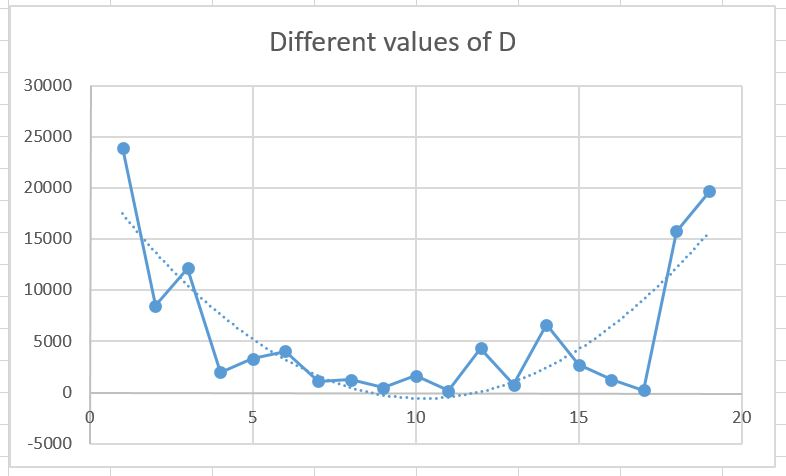
\includegraphics[width=\linewidth]{d.jpg}
  \caption{Different values of D.}
  \label{fig:result}
\end{figure}

In the figure \ref{fig:result}, we see that the time is big at the beginning and decreases to a optimum value of D before the time increases again. The total runtime is on the Y axes and the x axes is the number of runs. Between each run, there is an increment of $500$ for each D. 

\begin{figure}[h!]
  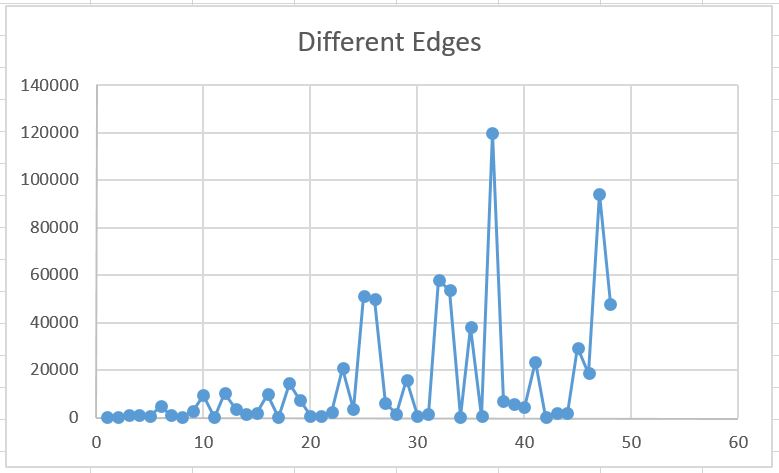
\includegraphics[width=\linewidth]{edge.jpg}
  \caption{Different sizes of edges.}
  \label{fig:result2}
\end{figure}

In figure \ref{fig:result2}, we can see that an increase of the edges result in longer runtime. The starting amount is $10000$ and the increasement is $500$ edges per run to a maximum of $40000$ edges.


\section{Discussion}
When we compare the two figures, \ref{fig:result2} and \ref{fig:result}, we see that increasing the edges will increase the runtime while the value of $D$ may worsen or improve the runtime. 
\\~\\
We notice that the value of $D$ has an optimum value for a given graph. While the edges only increase the runtime, the value of $D$ may improve the runtime instead.
We can see that the value of $D$ has a greater effect of the runtime when passed the optimum state.If we increase $D$ from its optimal value, the increase of $D$ will affect the runtime much more than the increase of the total edges in the graph.
\\~\\
PSEUDO of BIG O:\\
$
Worst case = vertices.length $*$ (adjesont.size $*$ log_d(vertices.length) + log_d(vertices.length))
$\\~\\
The implementation is crucial in an algorithm such as this one. This due to the fact that a faulty implementation, thinking about datastructsurs and functions, may and will affect the algorithms runtime to a degree where the result will be computed at a rate that is unusable. We noticed this behaviour from our previous implementations of this algorithm.
%%% End document
\end{document}
